\chapter{Gradio Application}
To demonstrate the model's capabilities and visualize the results interactively, we have developed a web application that integrates some of the previously mentioned features into a user-friendly interface using the Gradio framework. The application is designed with two main modules: the first for image segmentation, and the second for an AI assistant chatbot that helps users interact with vegetation and high-voltage network coordinates.
\section{Image Segmentation Module}
\begin{figure}[H]
 \centering
 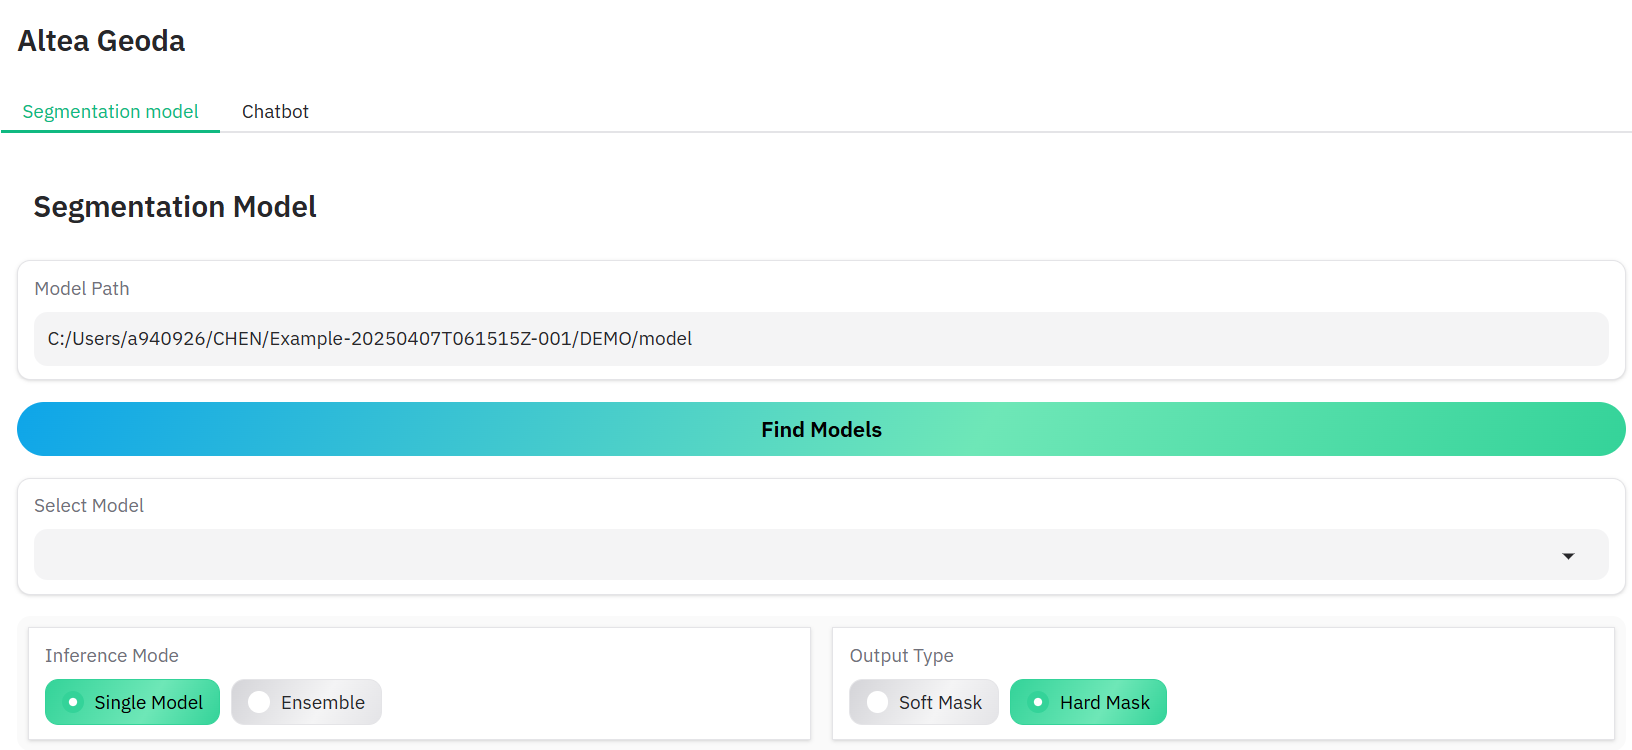
\includegraphics[scale=0.55]{IMAGENES/Gradio_app_segmentation1.png}
 \captionsetup{font=large}
 \caption {Gradio application (Image segmentation module).}
\end{figure}
In this module, users can upload a custom image and visualize the segmentation results directly in the browser. To perform inference, the user needs to specify the path to the directory where the model weights are stored. The pre-trained weights can be downloaded from the provided link [26], which contains six pre-trained models. Each model is named according to the dataset it was trained on, along with its corresponding training and testing accuracy. Users can either select a specific model for prediction or use an ensemble of all models for more robust results. Additionally, the application offers an option to choose the output type: Soft mask (outputs the raw probability map generated by the model) or Hard mask (Outputs a binary mask obtained by thresholding the soft mask at 0.5). There are no strict restrictions on the input image size or format, as the application automatically resizes the image to 512 x 512 pixels, which is the required input size for the model. However, for optimal performance, we recommend using images with dimensions close to 1024 x 1024 to 2048 x 2048 pixels, as these sizes match the training data.
\begin{figure}[H]
 \centering
 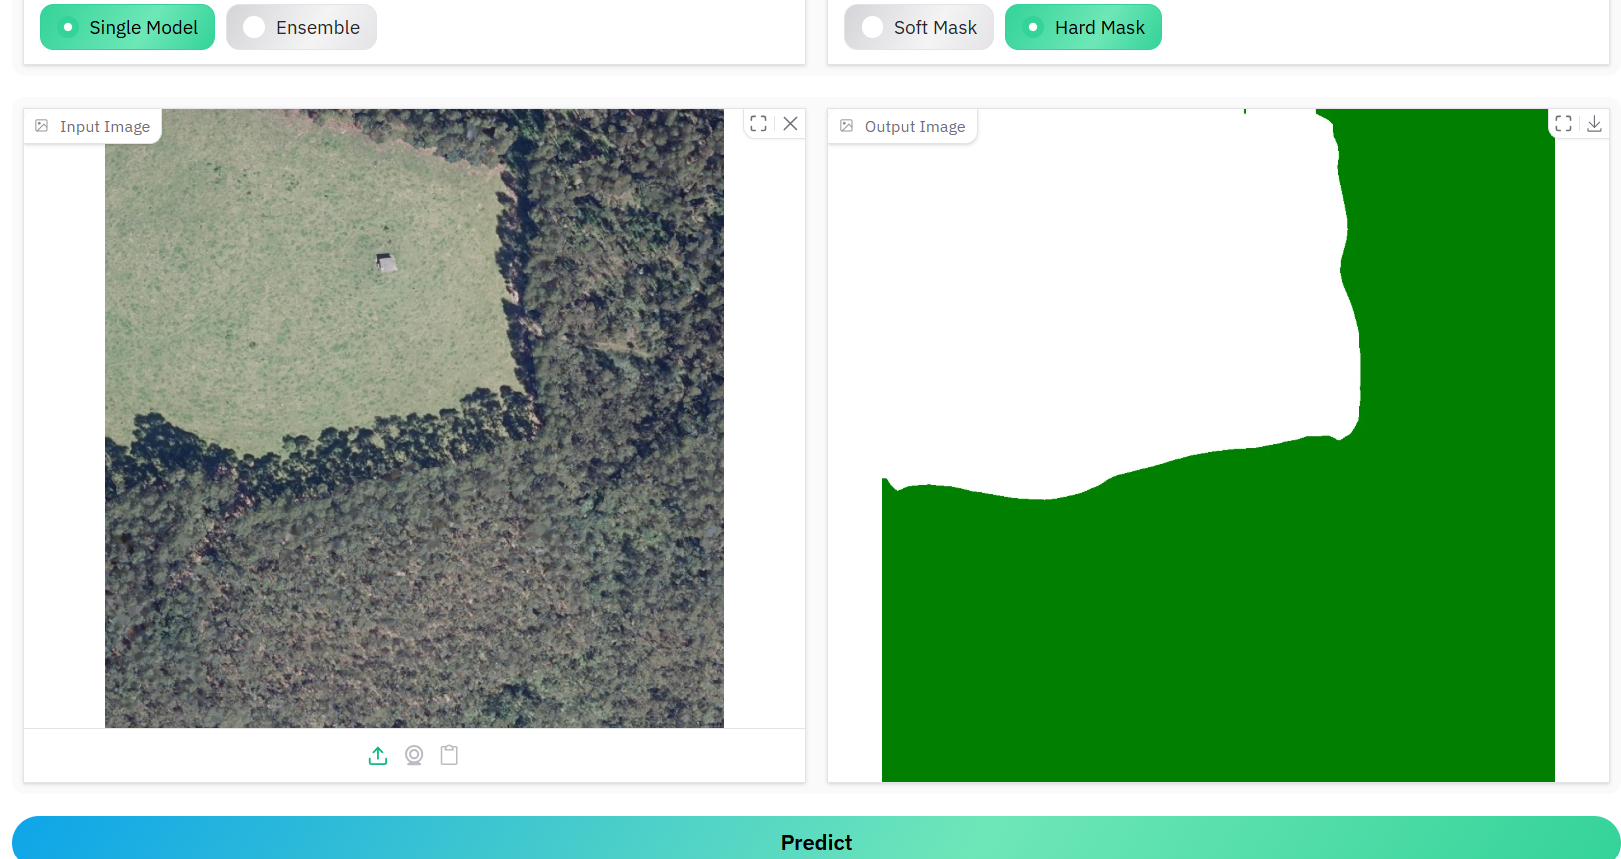
\includegraphics[scale=0.55]{IMAGENES/Gradio_app_segmentation2.png}
 \captionsetup{font=large}
 \caption {Gradio application (Image segmentation module).}
\end{figure}

\section{Ai Agent Assistant}
The second module is a chatbot assistant to interact with the coordinates of vegetation and high-voltage network. We provided all of our prediction results as coordinates stored in a CSV file, which contains 70 tiles in the Cantabria region, with each tile assigned a unique ID. Users can perform various queries through the chatbot to generate vegetation distribution, intersection or risk zone graphs. These queries can be made using either the tile ID, a specific location name or address.

\subsection{How the Chatbot Works}
The chatbot is built using an agent framework (LangGraph). An AI agent in this context refers to a language-model-powered system that can interact with external tools or environments and perform actions autonomously to achieve different objectives. In this application, we implemented a single agent with access to three primary tools:
\begin{itemize}
    \item \textbf{Display graph tool}: Displays graphs for a specific region based on the ID provided by the user.
    \item \textbf{Geocode tool}: Retrieves geographical coordinates based on a location name or address.
    \item \textbf{Get-id tool}: Finds the tile ID corresponding to a set of coordinates.
\end{itemize}
\textbf{Example Query}:\\
If the user asks:
"Display the intersection graph for Maliaño"
\begin{figure}[H]
 \centering
 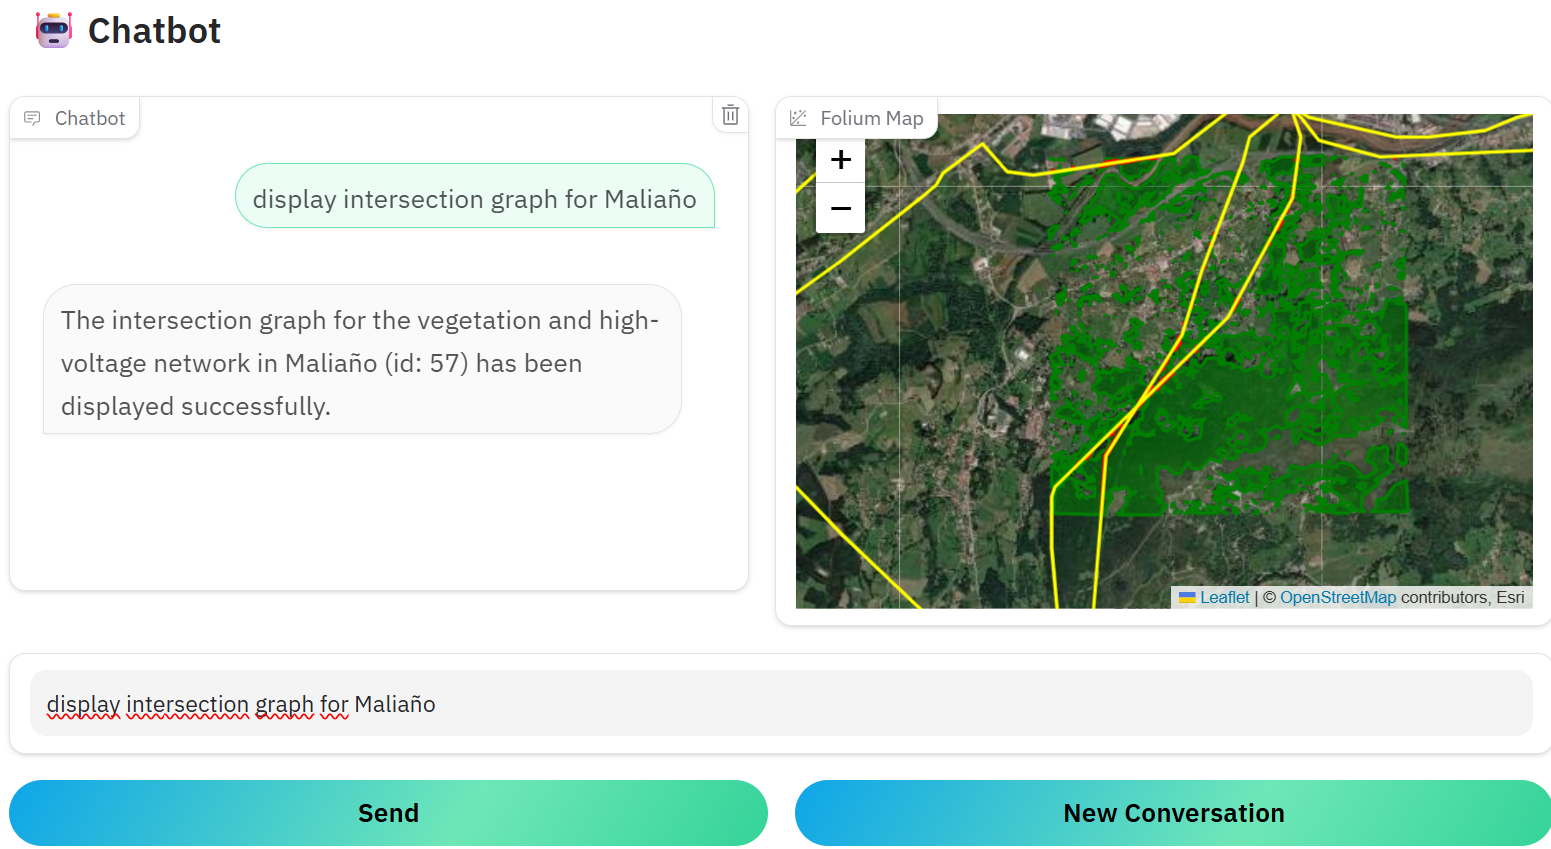
\includegraphics[scale=0.55]{IMAGENES/Gradio_app_chatbot.png}
 \captionsetup{font=large}
 \caption {Gradio Application (AI Agent Module): The module consists of two components. On the left, the user can view the chat history with the agent, and on the right, the user can view the queried graph on an interactive map.}
\end{figure}



the agent will follow these steps:
\begin{itemize}
    \item Call \textbf{Geocode tool} to retrieve the coordinates of "Maliaño".
    \item Call \textbf{Get-id tool} to determine the tile ID associated with those coordinates.
    \item Call \textbf{Display graph tool} to generate and display the vegetation distribution graph for the corresponding tile.
\end{itemize}
Beyond the basic query functionality, the chatbot supports advanced options, such as: Modifying the buffer size around high-voltage lines when generating intersection graphs. Or retrieving the addresses of the risk zone with largest area:

\begin{figure}[H]
 \centering
 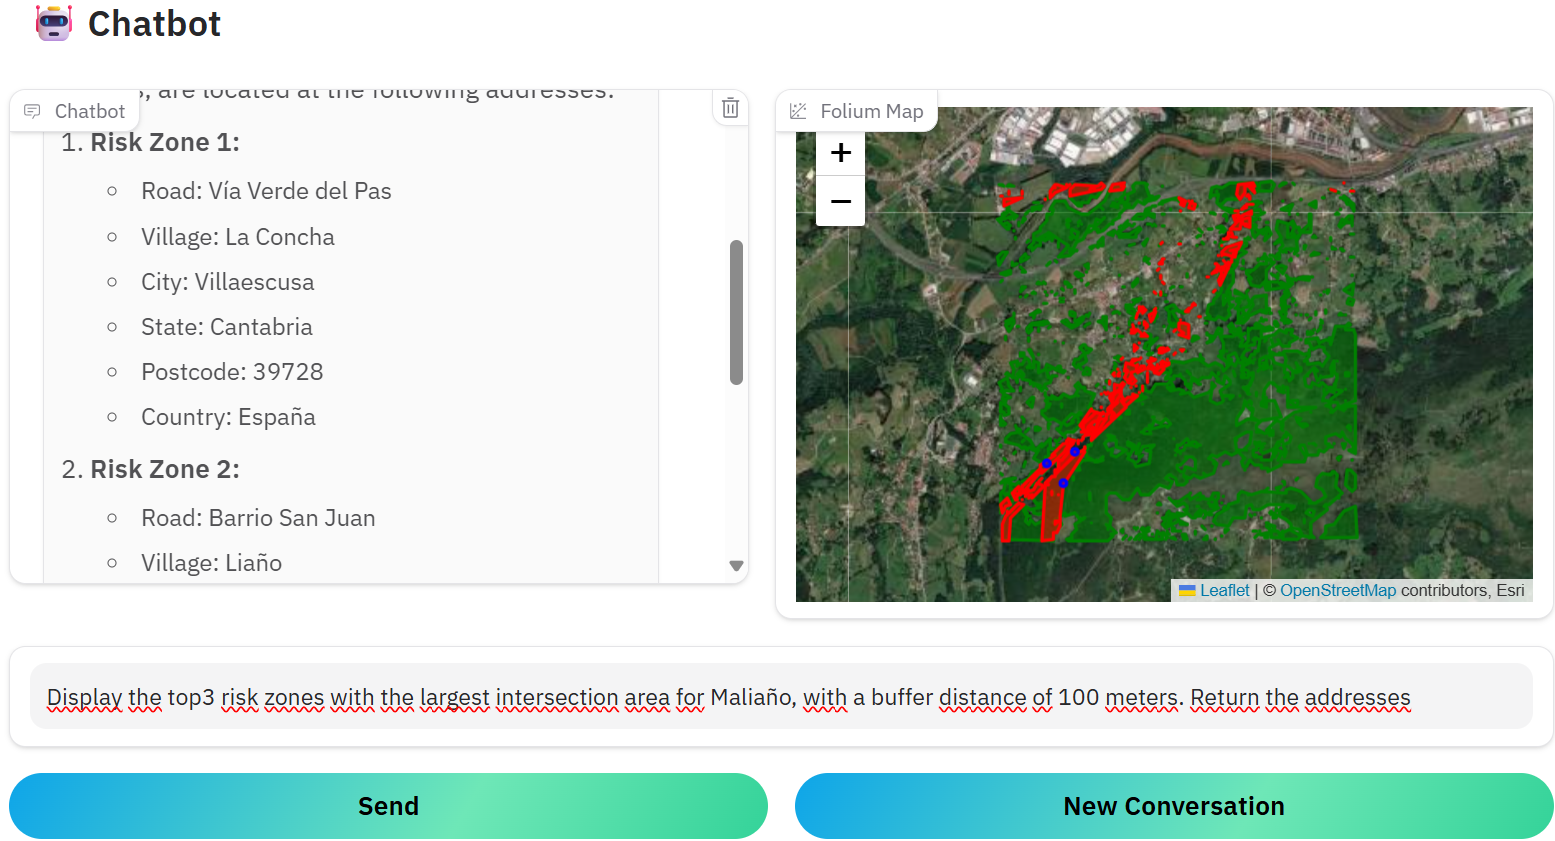
\includegraphics[scale=0.37]{IMAGENES/Gradio_app_chatbot2.png}
 \captionsetup{font=large}
 \caption {Gradio Application (AI Agent Module)}
\end{figure}

In this example, the buffer size is set to 100 meters, illustrating that the agent allows dynamic adjustment of this parameter. Additionally, the addresses of the top 3 zones with the largest intersection areas are displayed in the chat history.\\






